Изначально искусственные нейронные сети строились как модель коры головного мозга человека. 
В отличие от своего биологического аналога нейронная сеть как правило имеет дифференцируемые функции активации, необходимые 
для эффективного обучения в ходе обратного распространения ошибки.

\textit{Определение} \textbf{Функцией активации} в нейронной сети называется \textit{нелинейная} функция,
связывающая выходной сигнал и активацию нейрона 

На практике широко используются функции активации как сигмоида $\sigma$ , ReLU \cite{agarap2018deep} и GeLU \cite{hendrycks2016gaussian}

\begin{equation}
  \begin{aligned}
    & \sigma(x) = \frac{1}{1+\exp(-x)} \\
    &\text{ReLU}(x) = \min(0,x)p \\
    &\text{Tanh}(x) = \frac{e^{z}-e^{-z}}{e^{z}+e^{-z}} \\
    &\text{Gelu}(x) = \sigma(x) x 
  \end{aligned}
\end{equation}

Функция активации обычно вводится для добавления нелинейности в модель, что позволяет нейронной сети моделировать сложные нелинейные зависимости в данных.
Некоторые из распространенных функций активации включают в себя сигмоидальную функцию (\( \sigma \)), гиперболический тангенс (\( \tanh \)), ReLU (Rectified Linear Unit) и их вариации.


\textit{Определение} Перцептроном называется параметрическая математическая модель нейрона. Перцептрон
задается матрицей весов $W$, смещением $b$ и функцией активации $\sigma$
\begin{equation}
  \mathbf{y} = \sigma(W \mathbf{x} + \vec{b}),
\end{equation}

\begin{figure}[h]
  \centering
  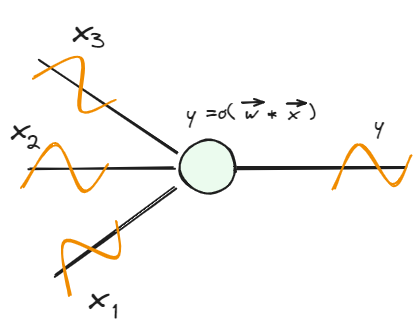
\includegraphics[width=0.5\textwidth]{assets/ml/nn/perceptron.excalidraw.png}
  \caption{Прямой процесс зашумления и обратный процесс коррекции ошибки \cite{stablediffusion}}
  \label{perceptron}
\end{figure}

\textit{Определение} \textbf{Нейронные сети} параметрическая аппроксимирующая модель, состоящая из слоев нейронов.

\begin{figure}[h]
  \centering
  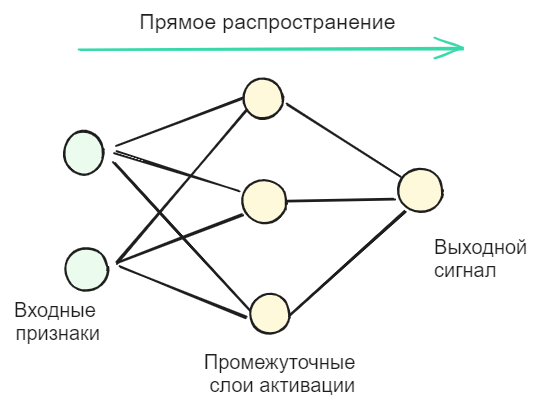
\includegraphics[width=0.5\textwidth]{assets/ml/nn/nn.excalidraw.png}
  \caption{Преобразование сигнала выполняется в промежуточных слоях активации в ходе прямого распространения сигнала}
  \label{neural_net}
\end{figure}

В случае многослойной нейронной сети, выходы нейронов одного слоя становятся входами для следующего слоя, образуя цепочку преобразований. 
Процесс распостранения через нейроны последовательных слоев называется прямым распространением (forward propagation).

Во время обучения модель минимизирует функцию потерь \( L \), 
которая оценивает разницу между предсказанным результатом $y_i$и истинным значением $y_i$:
\begin{equation}
  L = \frac{1}{N} \sum_{i=1}^{N} L(y_i, \hat{y}_i),
\end{equation}

обучение нейронной сети выполняется путем настройки весов \( \mathbf{w} \) и смещений \( b \) 
с использованием алгоритмов оптимизации, таких как градиентный спуск \ref{}. 
